\documentclass[a0paper,portrait]{baposter}

\usepackage[utf8]{inputenc}

\usepackage{amsmath}    
\usepackage{amsfonts}   
\usepackage{amsthm} 
\usepackage{caption}
\usepackage{graphicx}
\usepackage{paralist}
\usepackage{xcolor}

\definecolor{darktyrkis}{RGB}{0,143,149}

\begin{document}
\sffamily

\begin{poster}{
  columns=2,
	grid=false,
	borderColor=darktyrkis,
	headerColorOne=darktyrkis,
	headerColorTwo=darktyrkis,
	headerFontColor=white,
  headerheight=8em,
	boxColorOne=white,
  boxpadding=1em,
	headershape=rounded,
	headerfont=\Large\textsf,
	textborder=rounded,
	background=shadetb,
  bgColorOne=darktyrkis!10,
  bgColorTwo=darktyrkis!30,
	headerborder=open,
  boxshade=plain,
  eyecatcher=false
}
%%% Eye Catcher %%%%%%%%%%%%%%%%%%%%%%%%%%%%%%%%%%%%%%%%%%%%%%%%%%%%%%%%%%%%%%%
{
}
%%% Title %%%%%%%%%%%%%%%%%%%%%%%%%%%%%%%%%%%%%%%%%%%%%%%%%%%%%%%%%%%%%%%%%%%%%
{ \Huge Evolutionary optimization of machine learning pipelines}
%%% Authors %%%%%%%%%%%%%%%%%%%%%%%%%%%%%%%%%%%%%%%%%%%%%%%%%%%%%%%%%%%%%%%%%%%
{
  %\vspace{1em}
  \\Gabriela Suchopárová
}
%%% Logo %%%%%%%%%%%%%%%%%%%%%%%%%%%%%%%%%%%%%%%%%%%%%%%%%%%%%%%%%%%%%%%%%%%%%%
{
}

\small

%%% Abstract %%%%%%%%%%%%%%%%%%%%%%%%%%%%%%%%%%%%%%%%%%%%%%%%%%%%%%%%%%%%%%%%%%
\headerbox{Abstract}{name=abstract,column=0,row=0}{
\bfseries
We have developed a system that, for a given supervised
learning task, finds a suitable pipeline --- combination
of machine learning, ensembles and preprocessing methods --- using the developmental
genetic programming.
}

% last box to reference
\headerbox{OpenML-CC18 benchmark}{name=box4,column=0,span=2,above=bottom}{

\begin{minipage}{.5\textwidth}
  \centering
  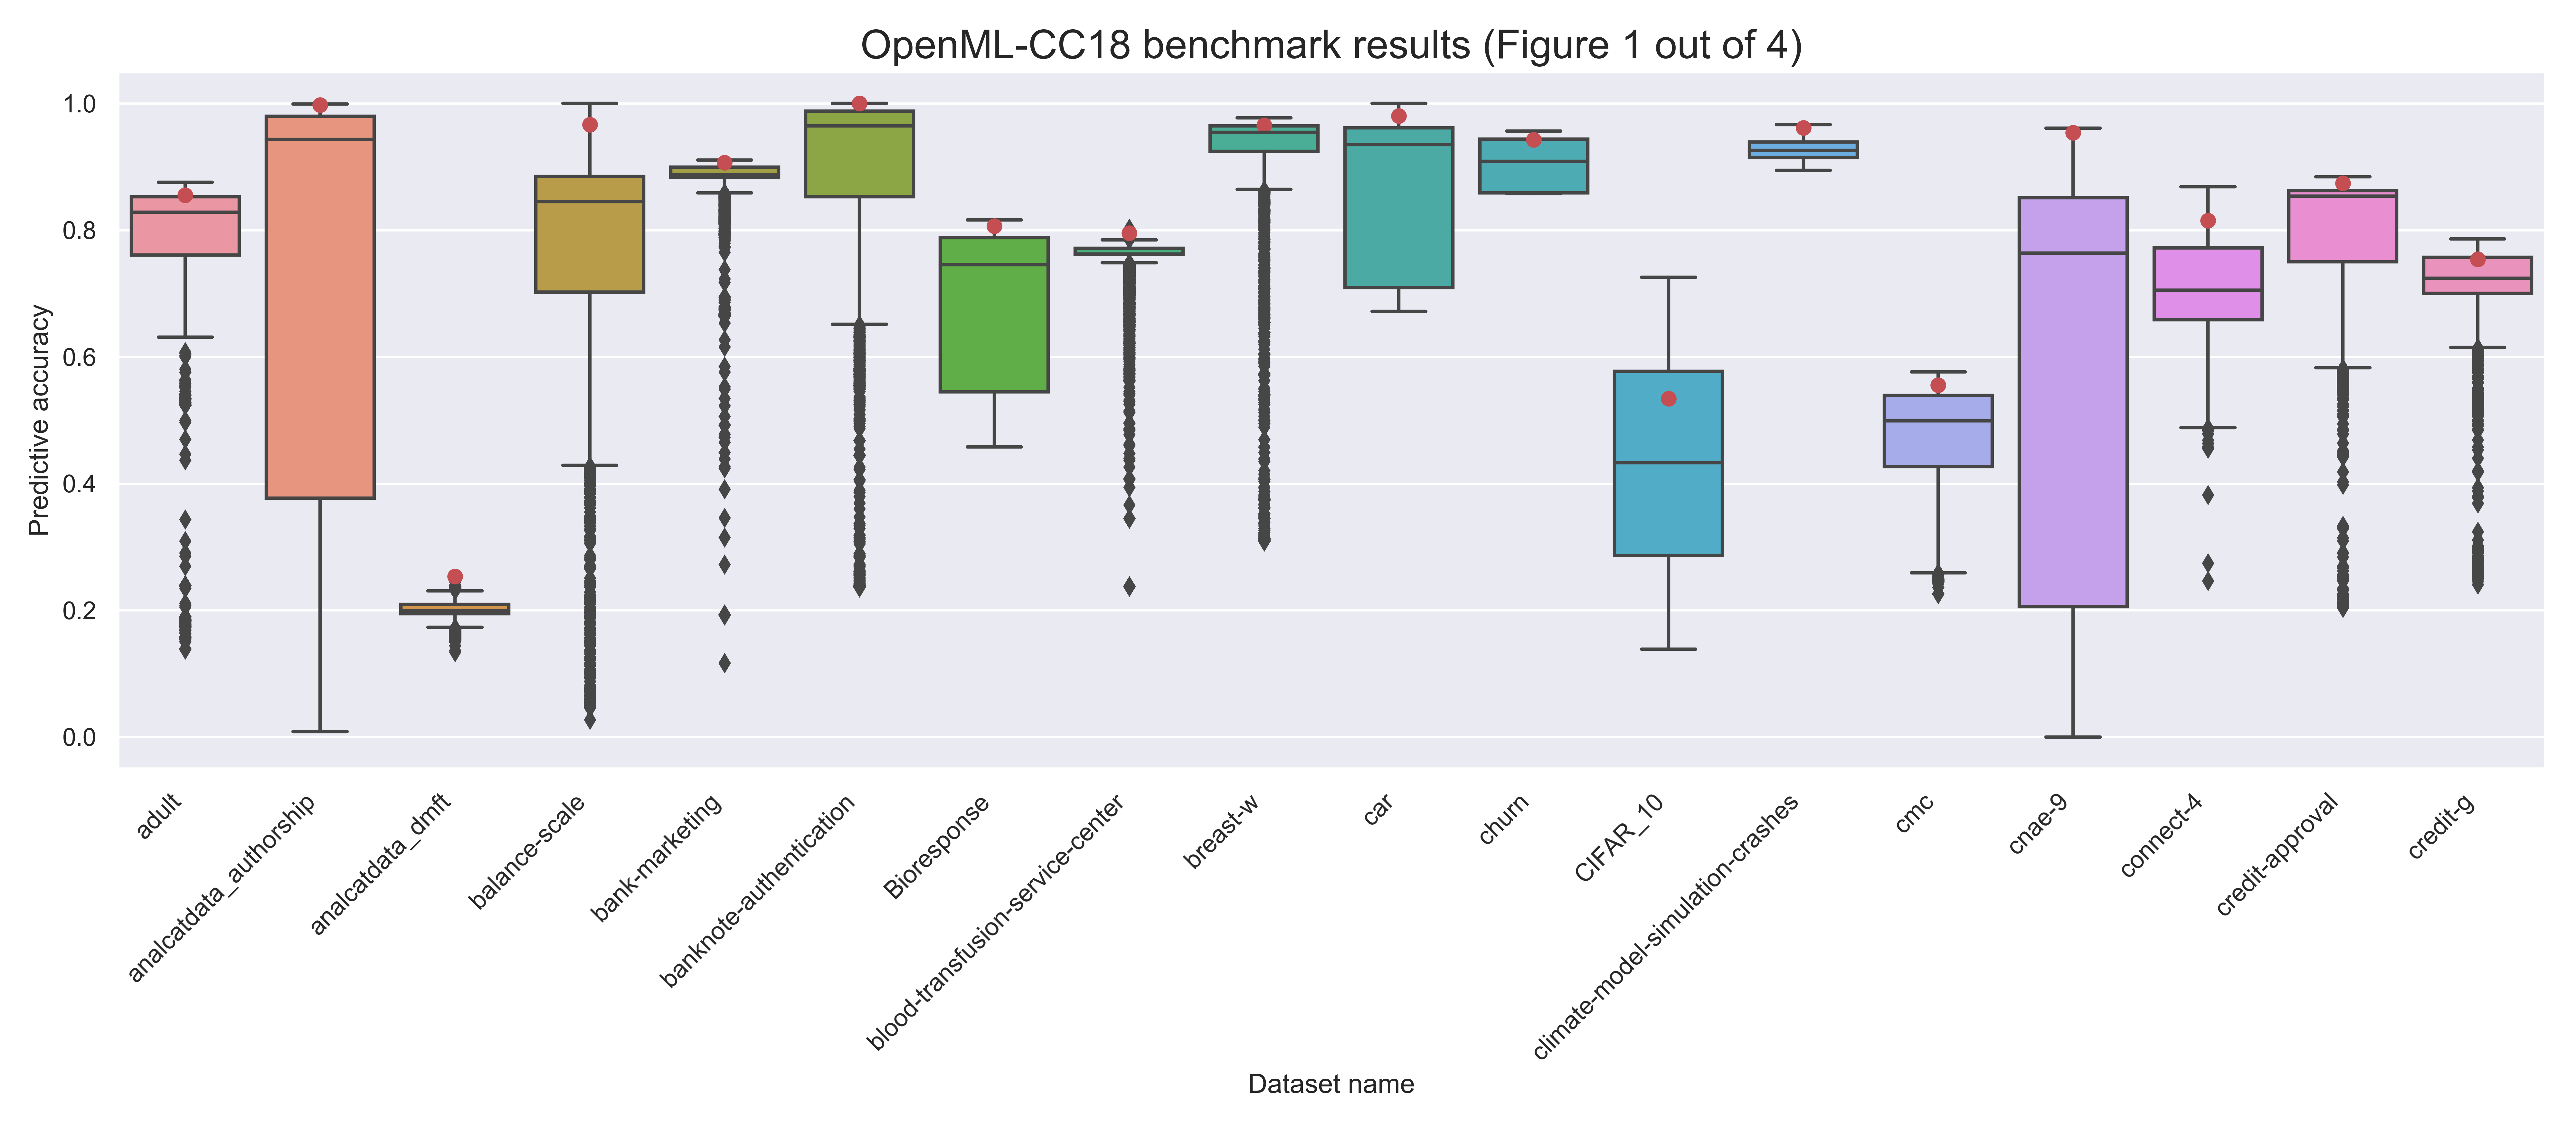
\includegraphics[width=0.8\linewidth]{../img/openml-boxplot0-hdpi.png}

\end{minipage}%
\begin{minipage}{.5\textwidth}
  \centering
  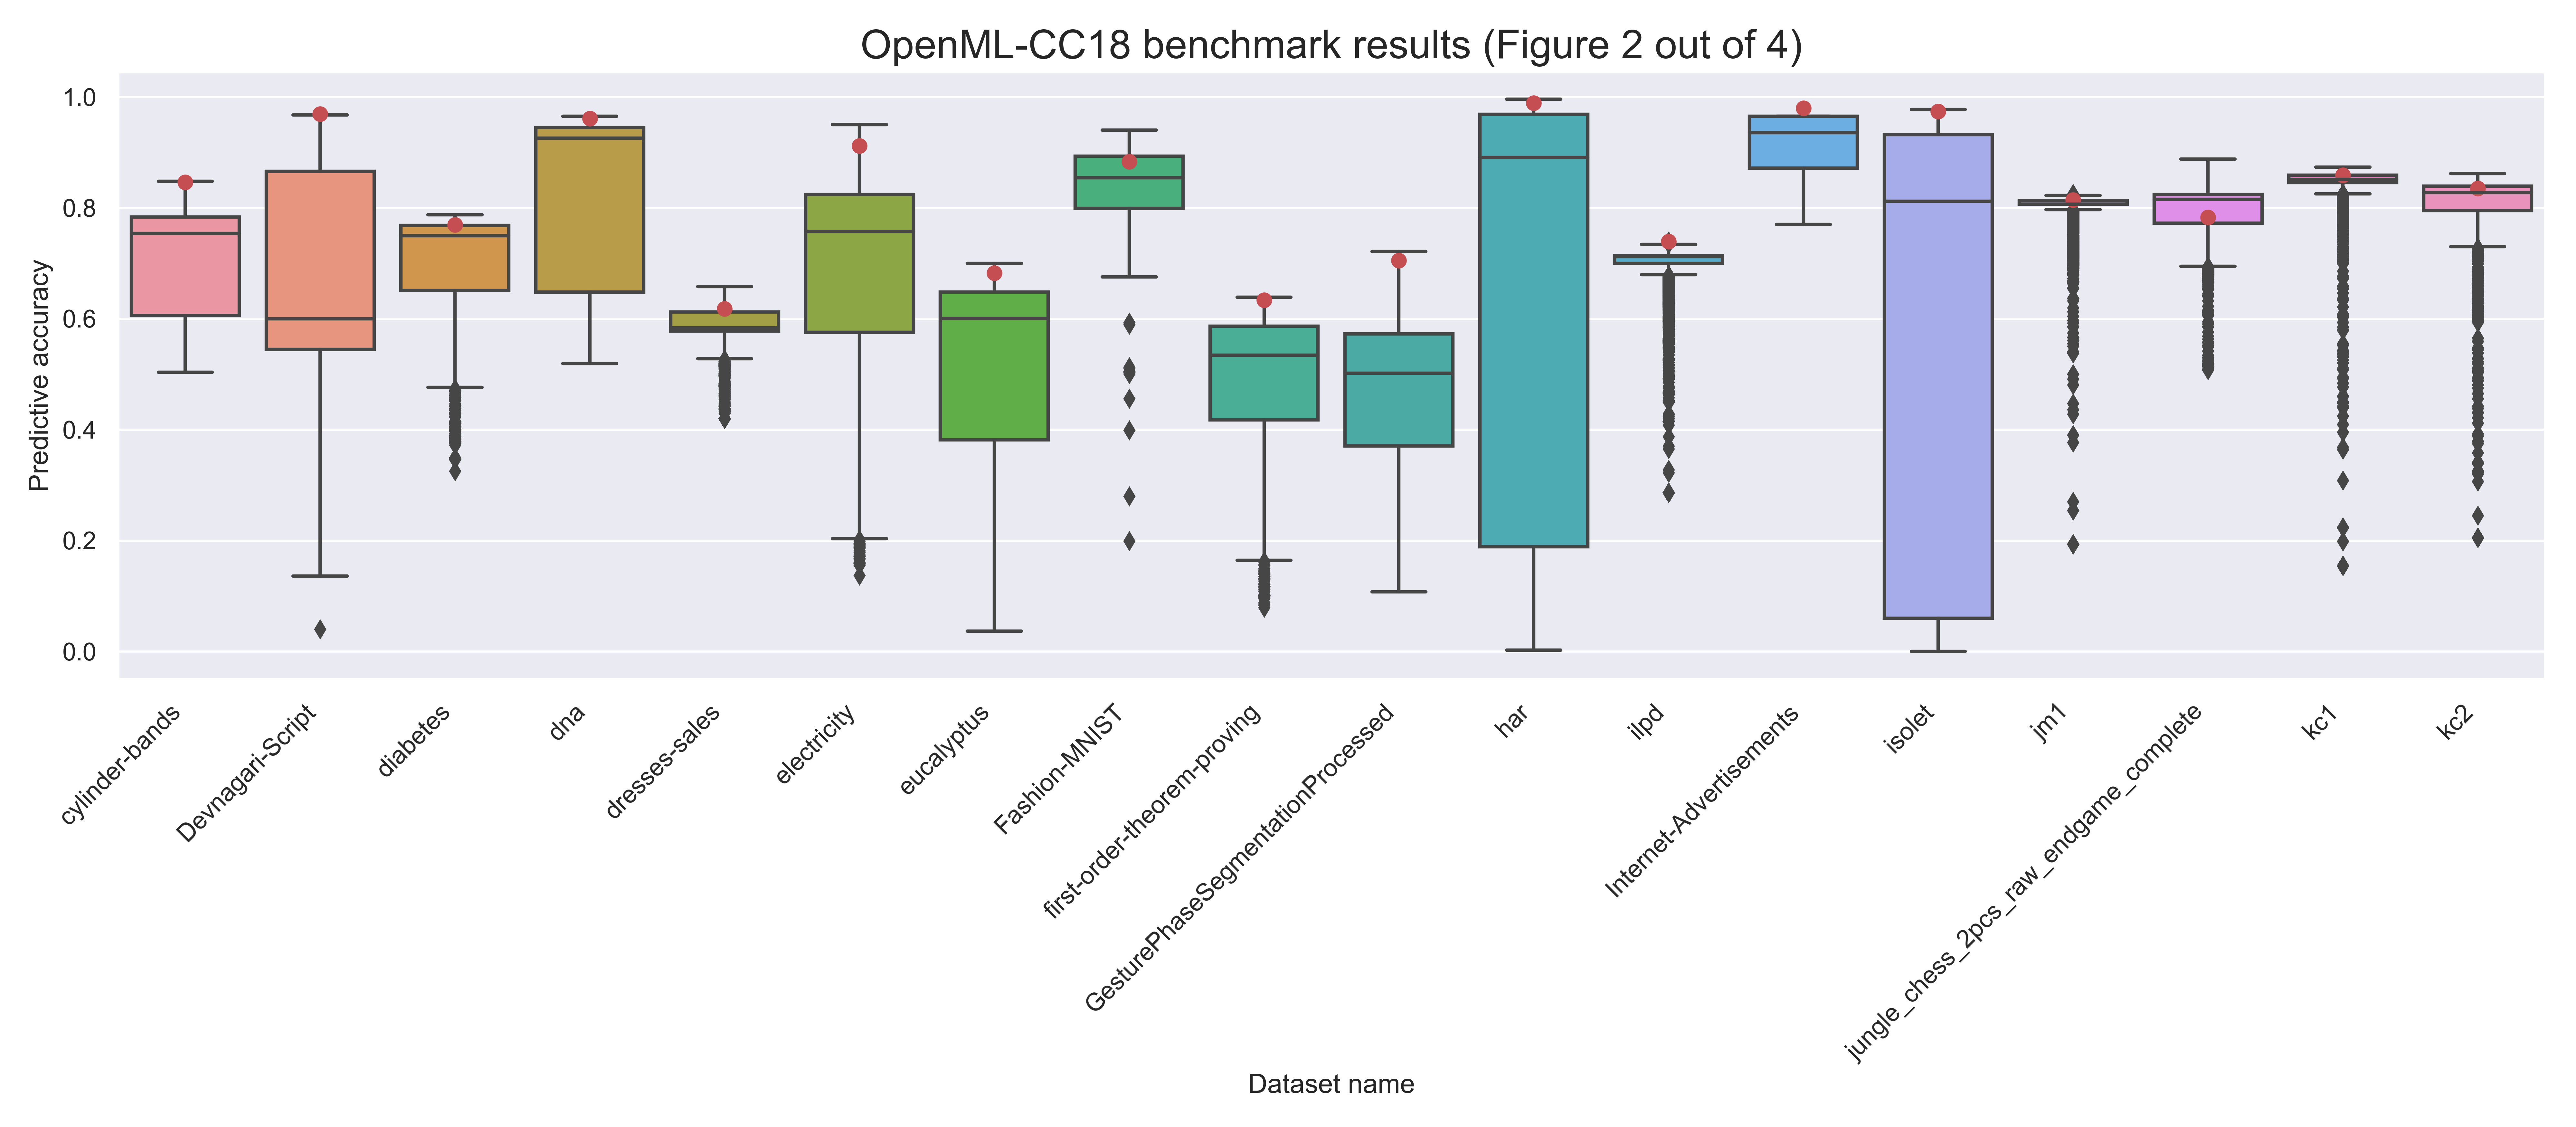
\includegraphics[width=0.8\linewidth]{../img/openml-boxplot1-hdpi.png}

\end{minipage}

\vspace{0.5em}

\begin{minipage}{.5\textwidth}
  \centering
  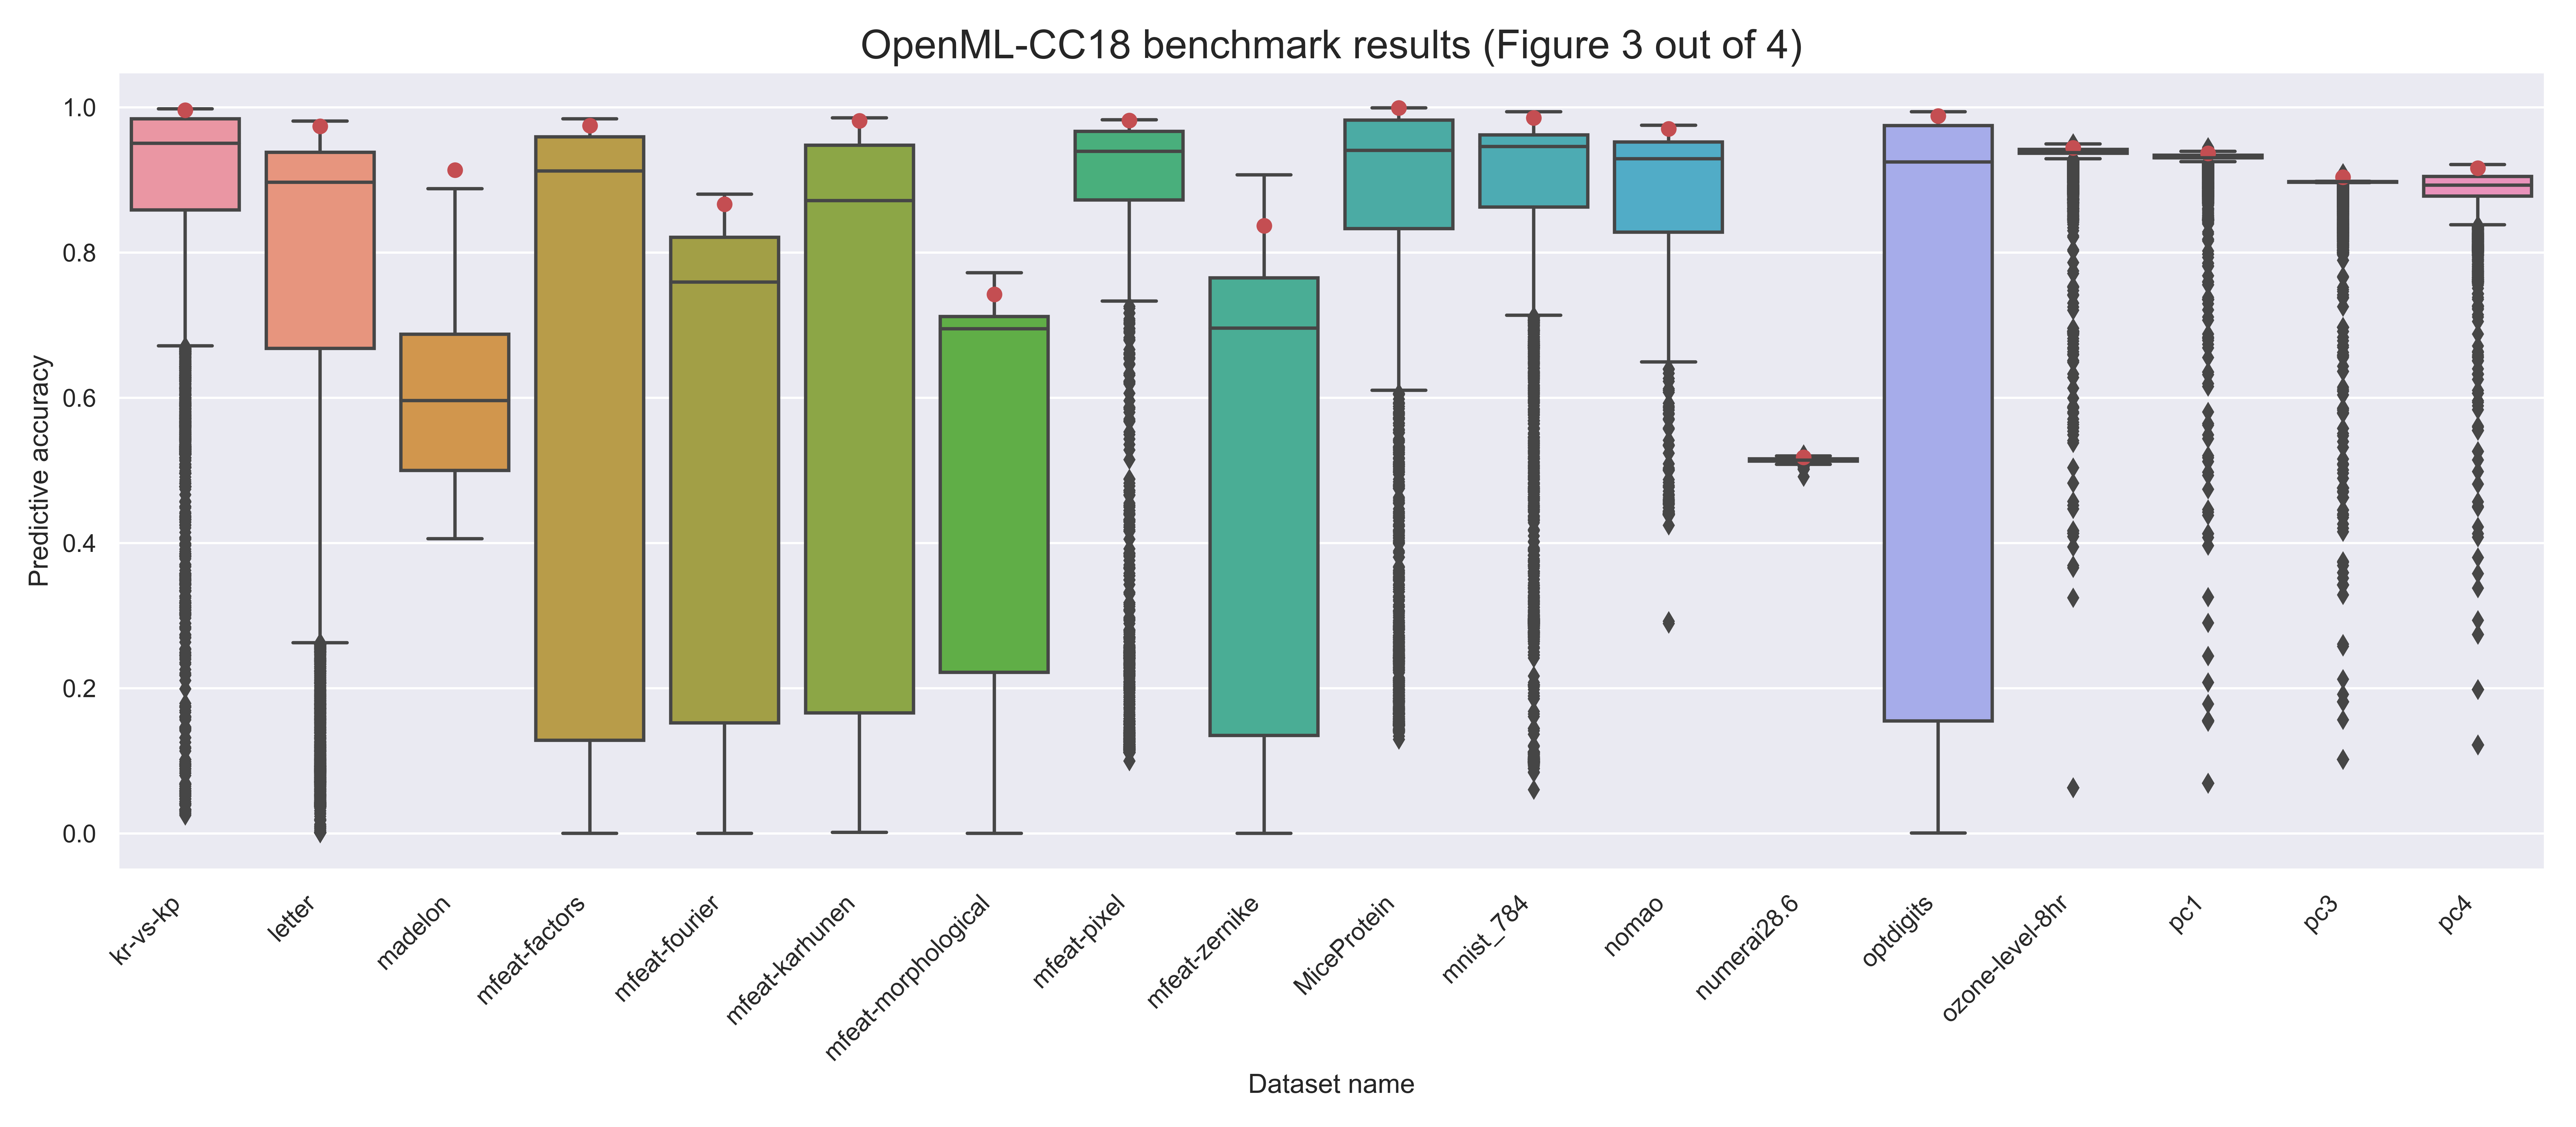
\includegraphics[width=0.8\linewidth]{../img/openml-boxplot2-hdpi.png}

\end{minipage}%
\begin{minipage}{.5\textwidth}
  \centering
  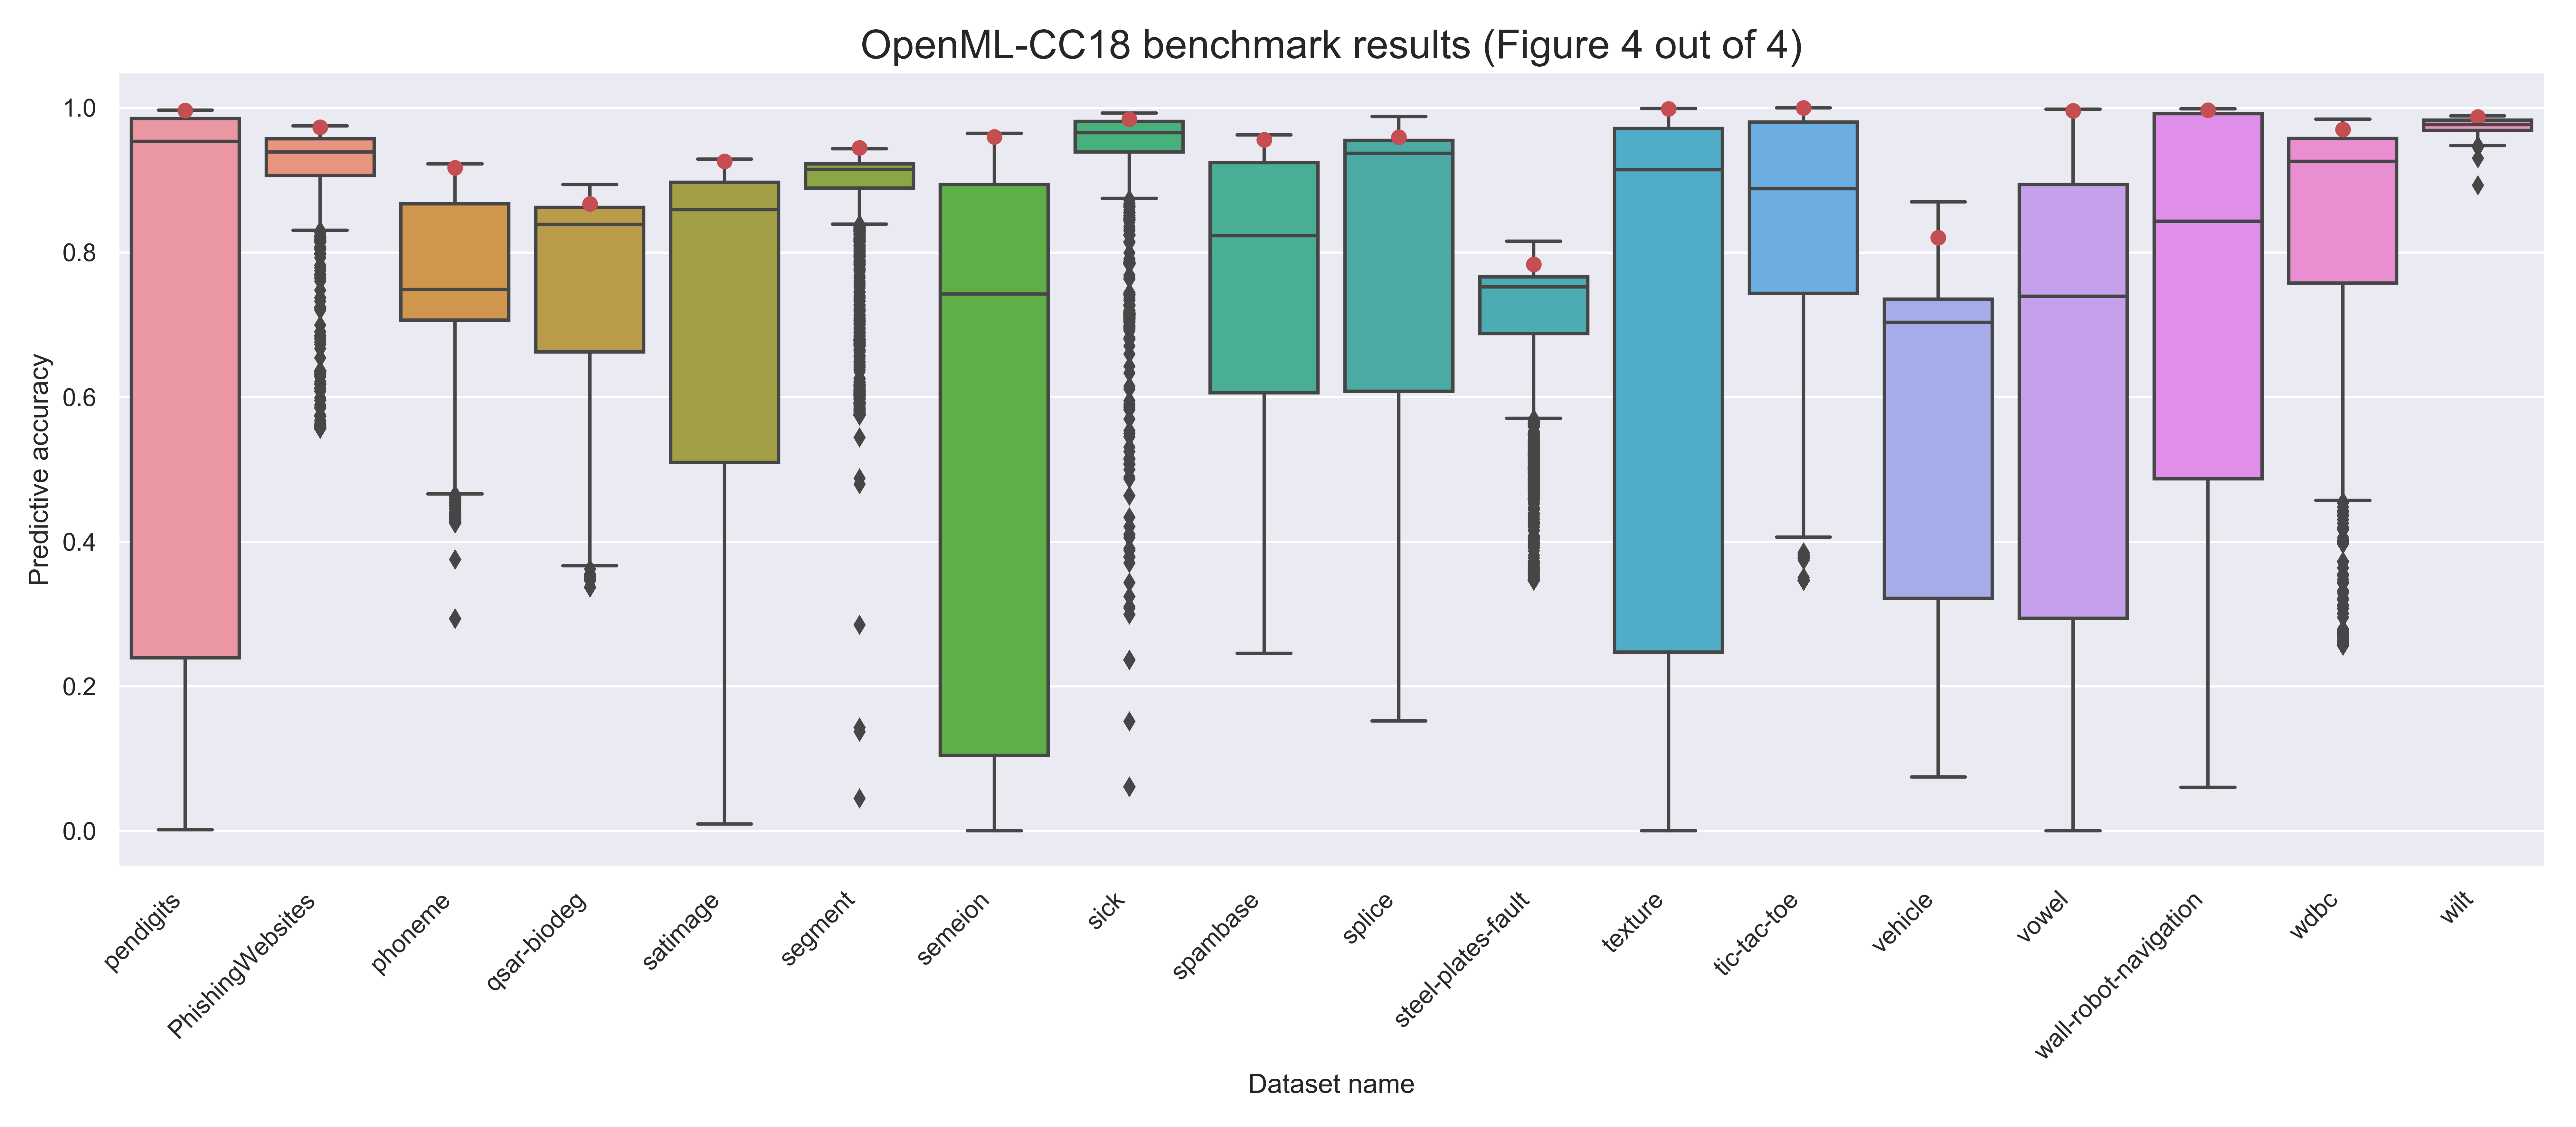
\includegraphics[width=0.8\linewidth]{../img/openml-boxplot3-hdpi.png}

\end{minipage}
}

\headerbox{AutoML}{name=box3,column=0, below=abstract}{
\begin{minipage}{\textwidth}
  \centering
  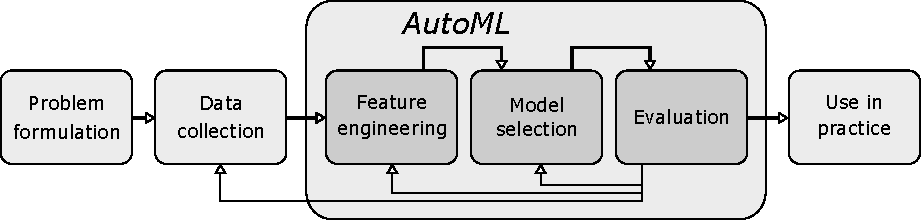
\includegraphics[width=0.7\linewidth]{../img/workflow-pdfa.pdf}
  \captionof{figure}{\sffamily Schema of a general workflow}
  \label{fig:workflow}
  \vspace{0.5em}
\end{minipage}

The AutoML systems aim to automatize a part of the machine learning workflow,
which is the process of selection of suitable feature
preprocessing methods and of a model with a particular hyperparameter setting.

\begin{minipage}{\textwidth}
  \centering
  \vspace{0.7em}
  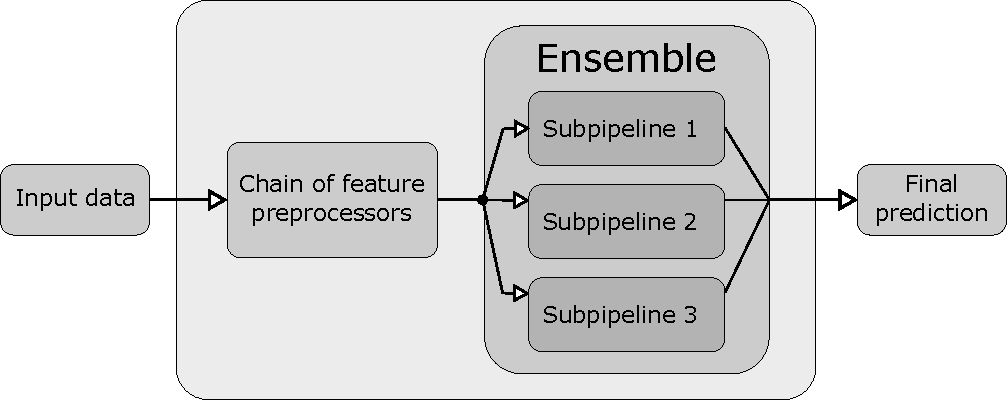
\includegraphics[width=0.65\linewidth]{../img/pipeline-pdfa.pdf}
  \captionof{figure}{\sffamily A more complex machine learning pipeline}
  \label{fig:pipeline}  
  \vspace{0.7em}
\end{minipage}

One of the tasks targeted by AutoML systems is \emph{pipeline optimization}. A machine
learning pipeline is composed from a chain of feature preprocessing methods and one
estimator. The estimator can be a simple method or an ensemble that contains one or more
base-estimators. Because a base-estimator can be a pipeline as well, a general pipeline
is a directed acyclic graph.
}

\headerbox{Our system}{name=box5,column=0, below=box3, above=box4}{
Our system aims to search for a pipeline that performs well on the given task. A
pipeline can be composed from both ensembles and feature preprocessing methods, but simple
methods are tried out as well.
}

%%% Box 2 %%%%%%%%%%%%%%%%%%%%%%%%%%%%%%%%%%%%%%%%%%%%%%%%%%%%%%%%%%%%%%%%%%%%%
\headerbox{Developmental GP}{name=box2,column=1}{
For pipeline optimization, we used the genetic programming (GP), which is a subfield
of evolutionary algorithms. 

\vspace{0.5em}
\begin{minipage}{\textwidth}

  \begin{minipage}{.5\textwidth}
    \centering
    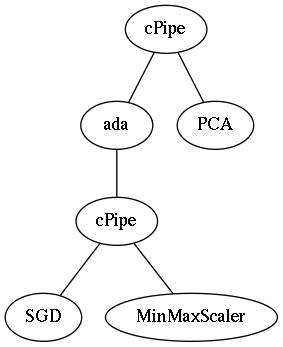
\includegraphics[width=0.45\linewidth]{../img/ada.png}

  \end{minipage}%
  \begin{minipage}{.5\textwidth}
    \centering
    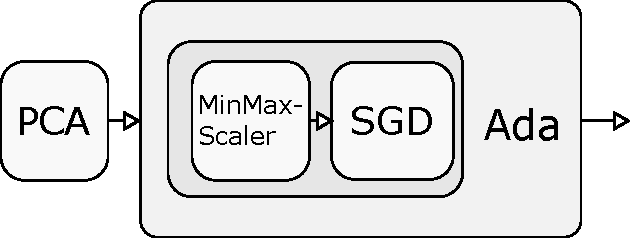
\includegraphics[width=0.8\linewidth]{../img/ada-pdfa.pdf}
  \end{minipage}
  
  \captionof{figure}{\sffamily Example of an encoded pipeline}
  \label{fig:encoding}
\end{minipage}
\vspace{0.5em}

We created a specific encoding that enables to convert pipelines in the form of a DAG into
a tree representation. Instead of directly encoding pipeline steps as nodes, we apply the
developmental GP, where the nodes represent \emph{operations} that create the pipeline.
An example of the encoding is shown in Figure \ref{fig:encoding}. The tree individual
contains instructions which construct the actual pipeline:

\vspace{0.5em}
\textbf{cPipe} --- create a pipeline with a preprocessor chain and an estimator
\begin{compactitem}
  \item[-] \textbf{ada} --- insert an AdaBoost ensemble with a base-estimator
  \begin{compactitem}
    \item[-] \textbf{cPipe} --- create a pipeline with a preprocessor chain
    \begin{compactitem}
      \item[-] \textbf{SGD} --- insert a SGD classifier
      \item[-] \textbf{MinMaxScaler} --- insert a MinMaxScaler
    \end{compactitem}
  
  \end{compactitem}
  
  \item[-] \textbf{PCA} --- insert the PCA preprocessor
\end{compactitem}
}

\headerbox{OpenML experiment}{name=box7,column=1,below=box2,above=box4}{
Our system was tested on the OpenML-CC18 benchmark, which is a suite of 72 datasets
available at OpenML. Each of the datasets is associated with a classification task,
the evaluation method is 10-fold cross-validation.
We present a comparison of our results with all other results uploaded to OpenML.
On most of the datasets our system performed in the upper quartile of
all results.
}

\end{poster}

\end{document}